\documentclass[11pt,dvipdfmx]{jarticle}

\usepackage{eee}
\usepackage{mymacros}

\newcounter{mycounter} % カウンタの宣言
\setcounter{mycounter}{0} % カウンタの初期化
\newcommand{\useMycounter}[1][]{\refstepcounter{mycounter}{#1}プログラム{\themycounter}:}

\begin{document}
% トップページを書く
\begin{jikkenTitle}
 \gakunen{3} % 学年を記述。この行で全体の枠を表示
 \numTitle{8}{LabVIEWによるトランジスタの4特性の自動測定} % 実験番号、タイトルを記述
 \subTitle{} % サブタイトルがあれば記述
 \jikkenbi{2024年11月7日(木)} % 実験日を記述
 \jikkenbiII{2024年11月21日(木)} % 実験日を記述(二日目がある場合。ない場合はこの行をコメントアウト)
 \kyoudou{} % 共同実験者名を記述
 \yoteibi{11/21}% 予定日を記述
 \hanNumberName{4}{3316}{関口 丞} % 班番号・学生番号・氏名を記述。この行でタイトルページの描画を終了
\end{jikkenTitle}

\section{目的}
本実験では、
\begin{itemize}
	\item トランジスタの入力/出力/電流伝達/電圧機関の諸特性図の概形が描けるようになる
	\item トランジスタの特性図が、hパラメータを求める方法を理解する
	\item 電圧と電流の関係式から、等価回路を求める方法を理解する
	\item LabVIEWを用いて、2端子対回路の電圧と電流を自動測定する方法を理解する
\end{itemize}
ことを目的とする。

\section{原理}
トランジスタはベース(B)、エミッタ(E)、コレクタ(C)の三端子を持つ半導体素子であり、各端子に流れる電流としてベース電流$i_b$、エミッタ電流$i_e$、コレクタ電流$i_c$が定義される。
実際の電圧・電流関係は非線形だが、回路設計では、トランジスタの動作を簡易に解析するため、\wfig{eqc}のような等価回路に基づく h パラメータを用いたモデルが利用される。
\begin{figure}[htb]
	\centering
	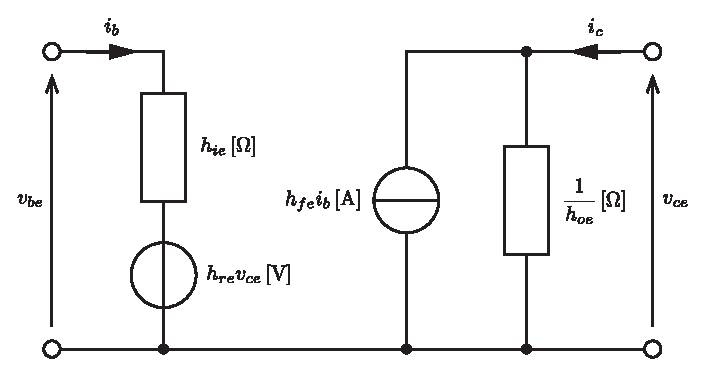
\includegraphics[width=90mm]{fig/eqc.eps}
	\caption{簡易等価回路}
	\label{fig:eqc}
\end{figure}
h パラメータは、次の線型方程式で表される。
\begin{equation}
	\begin{pmatrix}
		v_{be} \\
		i_c
	\end{pmatrix}
	=
	\begin{pmatrix}
		h_{ie} & h_{re} \\
		h_{fe} & h_{oe}
	\end{pmatrix}
	\begin{pmatrix}
		i_b \\
		v_{ce}
	\end{pmatrix}
	\label{eq:h_para}
\end{equation}
ここで、$h_{ie}\,[\Omega]$は入力インピーダンス、$h_{re}\,[-]$は電圧帰還率、$h_{fe}\,[-]$は電流増幅率、$h_{oe}\,[\mathrm{S}]$は出力アドミタンスと呼ばれるトランジスタの特性を示すパラメータである。

例えば、出力電流$i_c$は\weq{h_para}より、
\begin{equation}
	i_c = h_{fe}i_b + h_{oe}v_{ce}
	\label{eq:vce}
\end{equation}
で表されることから、素子特性値である$h_{fe}$、$h_{oe}$と、任意に決定できる$i_b$、$v_{ce}$によって決定されることが分かる。
この式に基づいて目的や仕様に沿うように回路の電圧や電流を決定していく回路設計が行われる。

4つのhパラメータは、\wfig{ch_h}に示すように\weq{h_para}右辺の微小変化$\Delta I_B$、$\Delta V_{CE}$に対する\weq{h_para}左辺の微小変化$\Delta I_C$、$\Delta V_{BE}$との比(傾き)によって表される。
\begin{figure}[H]
	\centering
	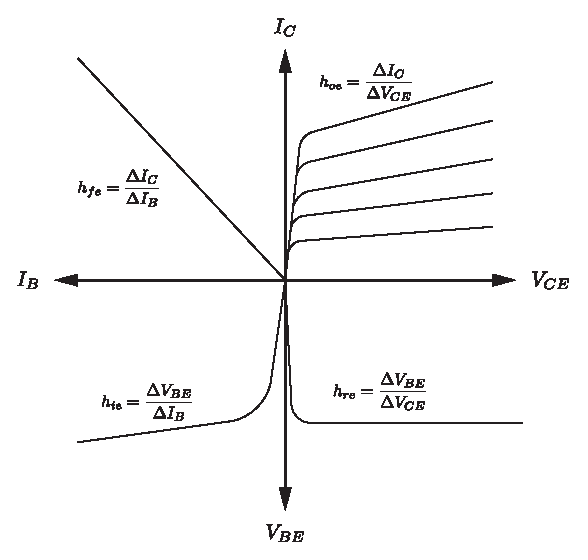
\includegraphics[width=80mm]{fig/hparam.eps}
	\caption{静特性曲線}
	\label{fig:ch_h}
\end{figure}
また、Hパラメータのような2端子回路の電圧と電流の4係数を2端子対パラメータと呼ぶ。2端子パラメータには他にYパラメータとZパラメータと呼ばれるものもある。
2端子対パラメータの内、電圧を電流で記述するものをZパラメータと呼ぶ。Zパラメータは\weq{Zパラメータ}に示す形で表される。
\begin{eqnarray}
	\begin{pmatrix}v_1\\v_2\end{pmatrix}&=&\begin{pmatrix}Z_{11}&Z_{12}\\Z_{21}&Z_{22}\end{pmatrix}\begin{pmatrix}i_1\\i_2\end{pmatrix}
	\label{eq:Zパラメータ}
\end{eqnarray}
またZパラメータはインピーダンスの次元[$\Omega$]をもつ。
2端子対パラメータの内、電流を電圧で記述するものをYパラメータと呼ぶ。Yパラメータは\weq{Yパラメータ}に示す形で表される。
\begin{eqnarray}
	\begin{pmatrix}i_1\\i_2\end{pmatrix}&=&\begin{pmatrix}Y_{11}&Y_{12}\\Y_{21}&Y_{22}\end{pmatrix}\begin{pmatrix}v_1\\v_2\end{pmatrix}
	\label{eq:Yパラメータ}
\end{eqnarray}
Yパラメータはアドミタンスの次元[S]を持つ。またYパラメータはZパラメータの逆行列になっている。
\section{実験}
	\subsection{使用器具}
		\wtab{使用器具}に本実験に用いた使用器具を示す。
		\begin{table}[H]
			\centering
			\caption{使用器具}
			\begin{tabular}{|c|c|c|c|}
			\hline
			器具名 & 型番 & 製造元 & シリアルナンバー \\ \hline\hline
			LabVIEW & / & NATIONAL INSTRUMENTS & / \\
			myRIO & 154294E-01L & NATIONAL INSTRUMENTS & MyRIO No.06 / \\
			myRIOブレッドボードアクセサリ & / & NATIONAL INSTRUMENTS & MyRIO No.06 \\ 
			ノートパソコン & /& iiyama & MyRIO-06 \\
			トランジスタ & 2N3904 & ON Semiconductor & / \\
			抵抗(100 k$\Omega $) & / & / & / \\
			抵抗 (470 $\Omega$) & / & / & / \\
			\hline
			\end{tabular}
			\label{tab:使用器具}
		\end{table}
	\subsection{比較演算とwhileループの演習}
			\begin{enumerate}
				\item \wfig{比較演算子とwhileループの演習プログラム}に示すプログラムを組んだ。
				\begin{figure}[H]
					\centering
					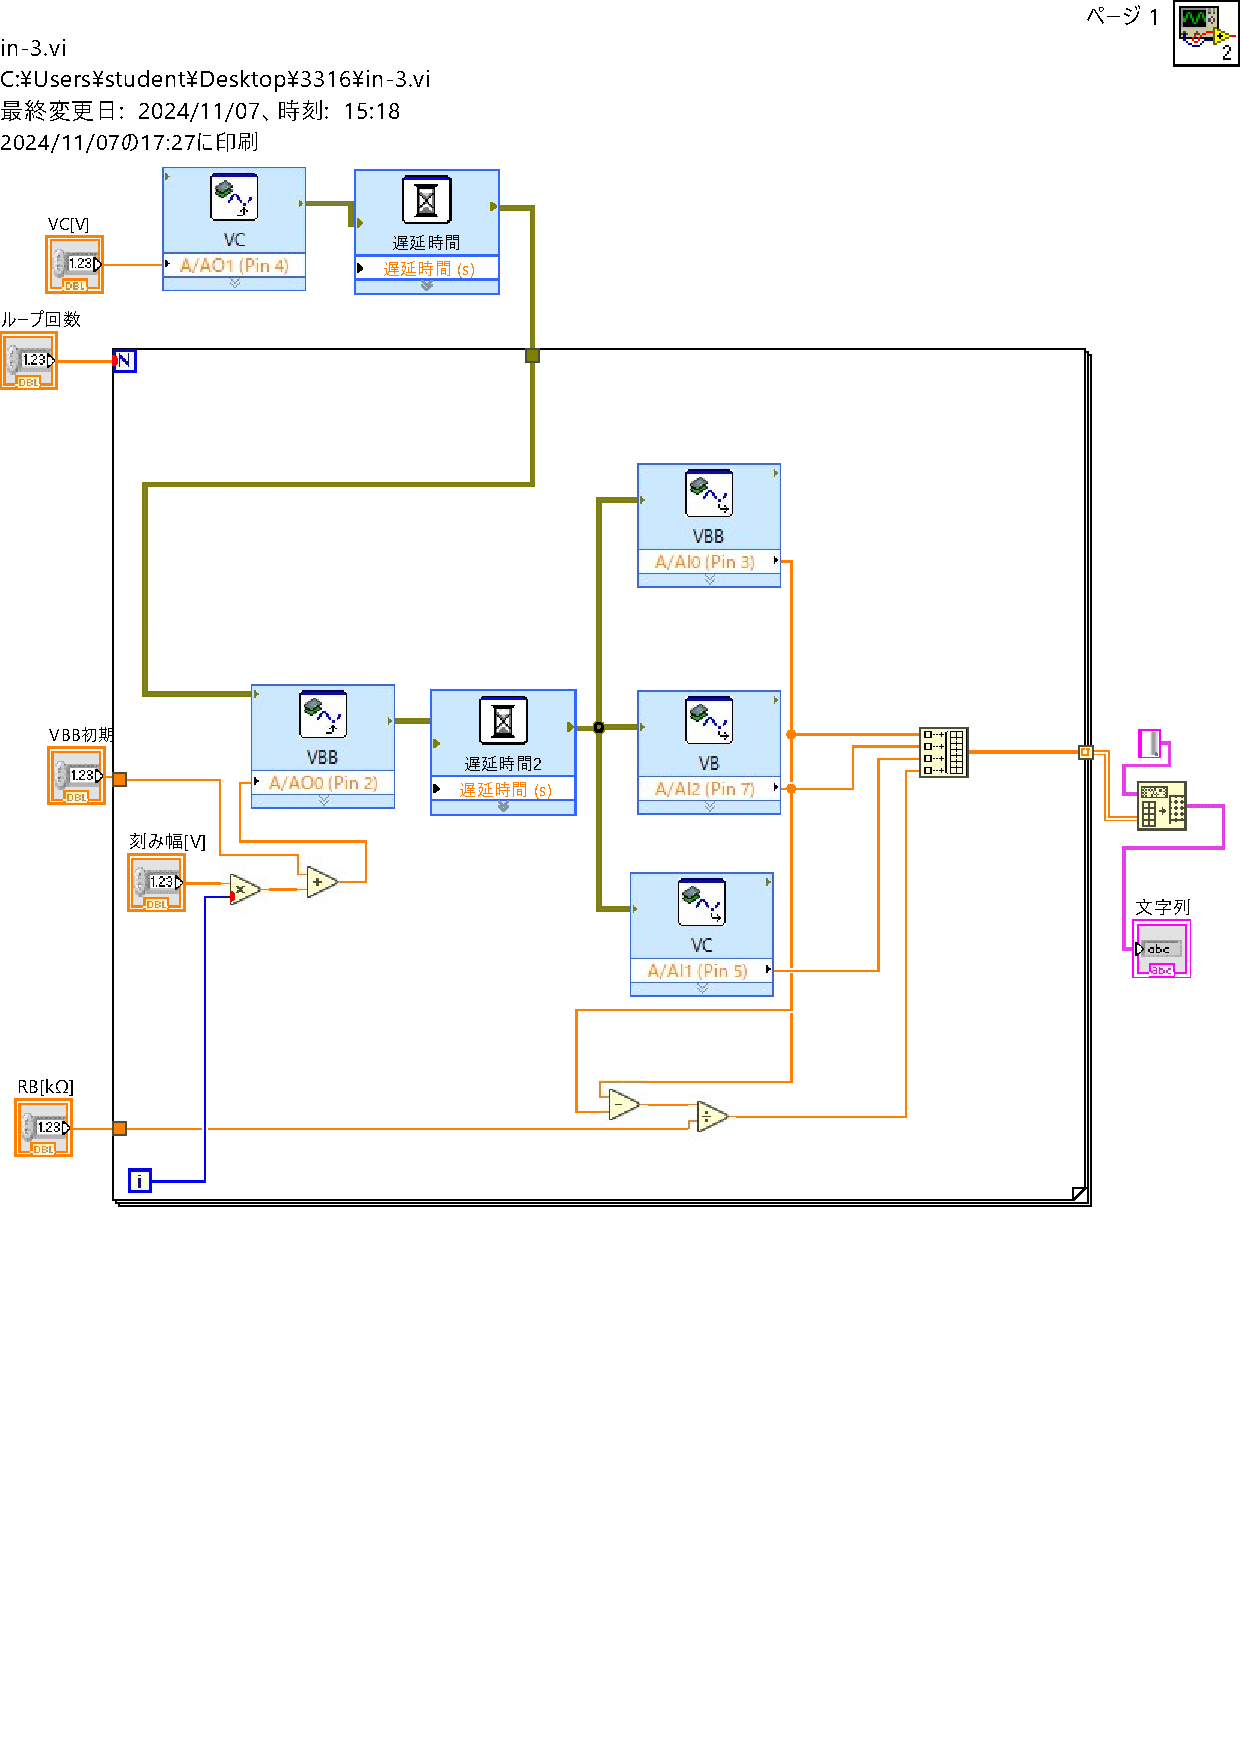
\includegraphics[scale=0.3]{fig/in-3.pdf}
					\caption{比較演算子とwhileループの演習プログラム}
					\label{fig:比較演算子とwhileループの演習プログラム}
				\end{figure}
				\item \wfig{比較演算子とwhileループの演習プログラム}の数値制御機に適当な値を入れ、動くか検証した。
				\item \wfig{比較演算子とwhileループの演習プログラム}のプログラムを刻み幅0.1と0.2でそれぞれ18回繰り返し測定を行うように設定し、動くか検証した。
			\end{enumerate}
	\subsection{BJTの入力特性図}
		\begin{enumerate}
			\item \wfig{入力特性の測定回路}の$R_B$に用いる抵抗の抵抗値をテスターで測定した。
			\item \wfig{入力特性の測定回路}に示す測定回路をブレッドボード上に組んだ。
			\begin{figure}[H]
				\centering
				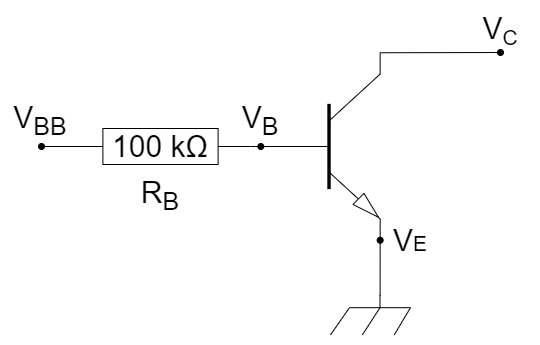
\includegraphics[scale=0.3]{fig/BJT入力特性測定回路.drawio.png}
				\caption{入力特性の測定回路}
				\label{fig:入力特性の測定回路}
			\end{figure}
			\item 測定回路とmyRIOの端子を\wtab{入力特性の測定回路とmyRIOの接続}に示すように接続した。
			\begin{table}[H]
				\centering
				\caption{入力特性の測定回路とmyRIOの接続}
				\begin{tabular}{ccc}
				\hline
				回路図の記号 & &接続ポート \\ \hline\hline
				$V_{BB}$ & - & AI0,AO0 \\
				$V_B$ & - & AI2 \\
				$V_C$ & - & AI1,AO1 \\
				$V_E$ & - & GND \\
				$GND$ & - & AIのGND \\
				$GND$ & - & AOのGND \\
				\hline
				\end{tabular}
				\label{tab:入力特性の測定回路とmyRIOの接続}
			\end{table}
			\item \wfig{入力特性測定プログラム}に示すプログラムを組んだ。
			\item 変数を次のように設定し、$V_{BB}$,$V_C$が指定通りになっているか、また、$V_B$が0.7 V 程度になっていることを確認した。
			\begin{itemize}
				\item $V_C=4$ V
				\item $V_{BB}=3.4$ V
			\end{itemize}
			\item \wfig{入力特性測定プログラム}のプログラムを別名で保存し、以下の要項で自動測定するように修正し、実行した。
			\begin{itemize}
				\item $V_{BB}$,$V_B$,$R_B$より$I_B$を算出。
				\item $I_B$を配列結合に加える。
				\item 測定結果(文字列)を1行4列で表示。
			\end{itemize}
			\item 上述のプログラムを別名で保存し、以下の要項で自動測定するように修正した。
			\begin{itemize}
				\item $V_{BB}$を 0 V から 3.4 V まで 0.2 V 刻みで変化させる。
				\item 各$V_{BB}$に対して、$V_C$,$V_{BB}$,$V_B$,$I_B$を測定する。
			\end{itemize}
			\item 測定結果をExcelで処理し、入力特性図として描画した。
		\end{enumerate}
	\subsection{BJT電流伝達特性}
	\label{sec:BJT電流伝達特性}
		\begin{enumerate}
			\item \wfig{電流伝達特性測定回路}の$R_C$に用いる抵抗の抵抗値をテスターで測定した。
			\item \wfig{電流伝達特性測定回路}に示す測定回路をブレッドボード上に組んだ。
			\item 測定回路とmyRIOの端子を\wtab{電流伝達特性の測定回路とmyRIOの接続}に示すように接続した。
			\begin{table}[H]
				\centering
				\caption{電流伝達特性の測定回路とmyRIOの接続}
				\begin{tabular}{ccc}
				\hline
				回路図の記号 & &接続ポート \\ \hline\hline
				$V_{BB}$ & - & AI0,AO0 \\
				$V_B$ & - & AI2 \\
				$V_{CC}$ & - & AI1,AO1 \\
				$V_C$ & - & AI3 \\
				$V_E$ & - & GND \\
				$GND$ & - & AIのGND \\
				$GND$ & - & AOのGND \\
				\hline
				\end{tabular}
				\label{tab:電流伝達特性の測定回路とmyRIOの接続}
			\end{table}
			\item \wfig{電流伝達特性測定プログラム}に示すように以下の要項で入力特性測定プログラムを修正した。
			\begin{itemize}
				\item ラベル$V_C$を$V_{CC}$に修正する。
				\item $V_{CC}$,$V_C$,$R_C$より$I_C$を算出する。
				\item $V_{BB}$を 0 V から 1.8 V まで 0.1 V 刻みで変化させる。
				\item 測定結果(文字列)を19行6列で表示。
			\end{itemize}
			\begin{figure}[H]
				\centering
				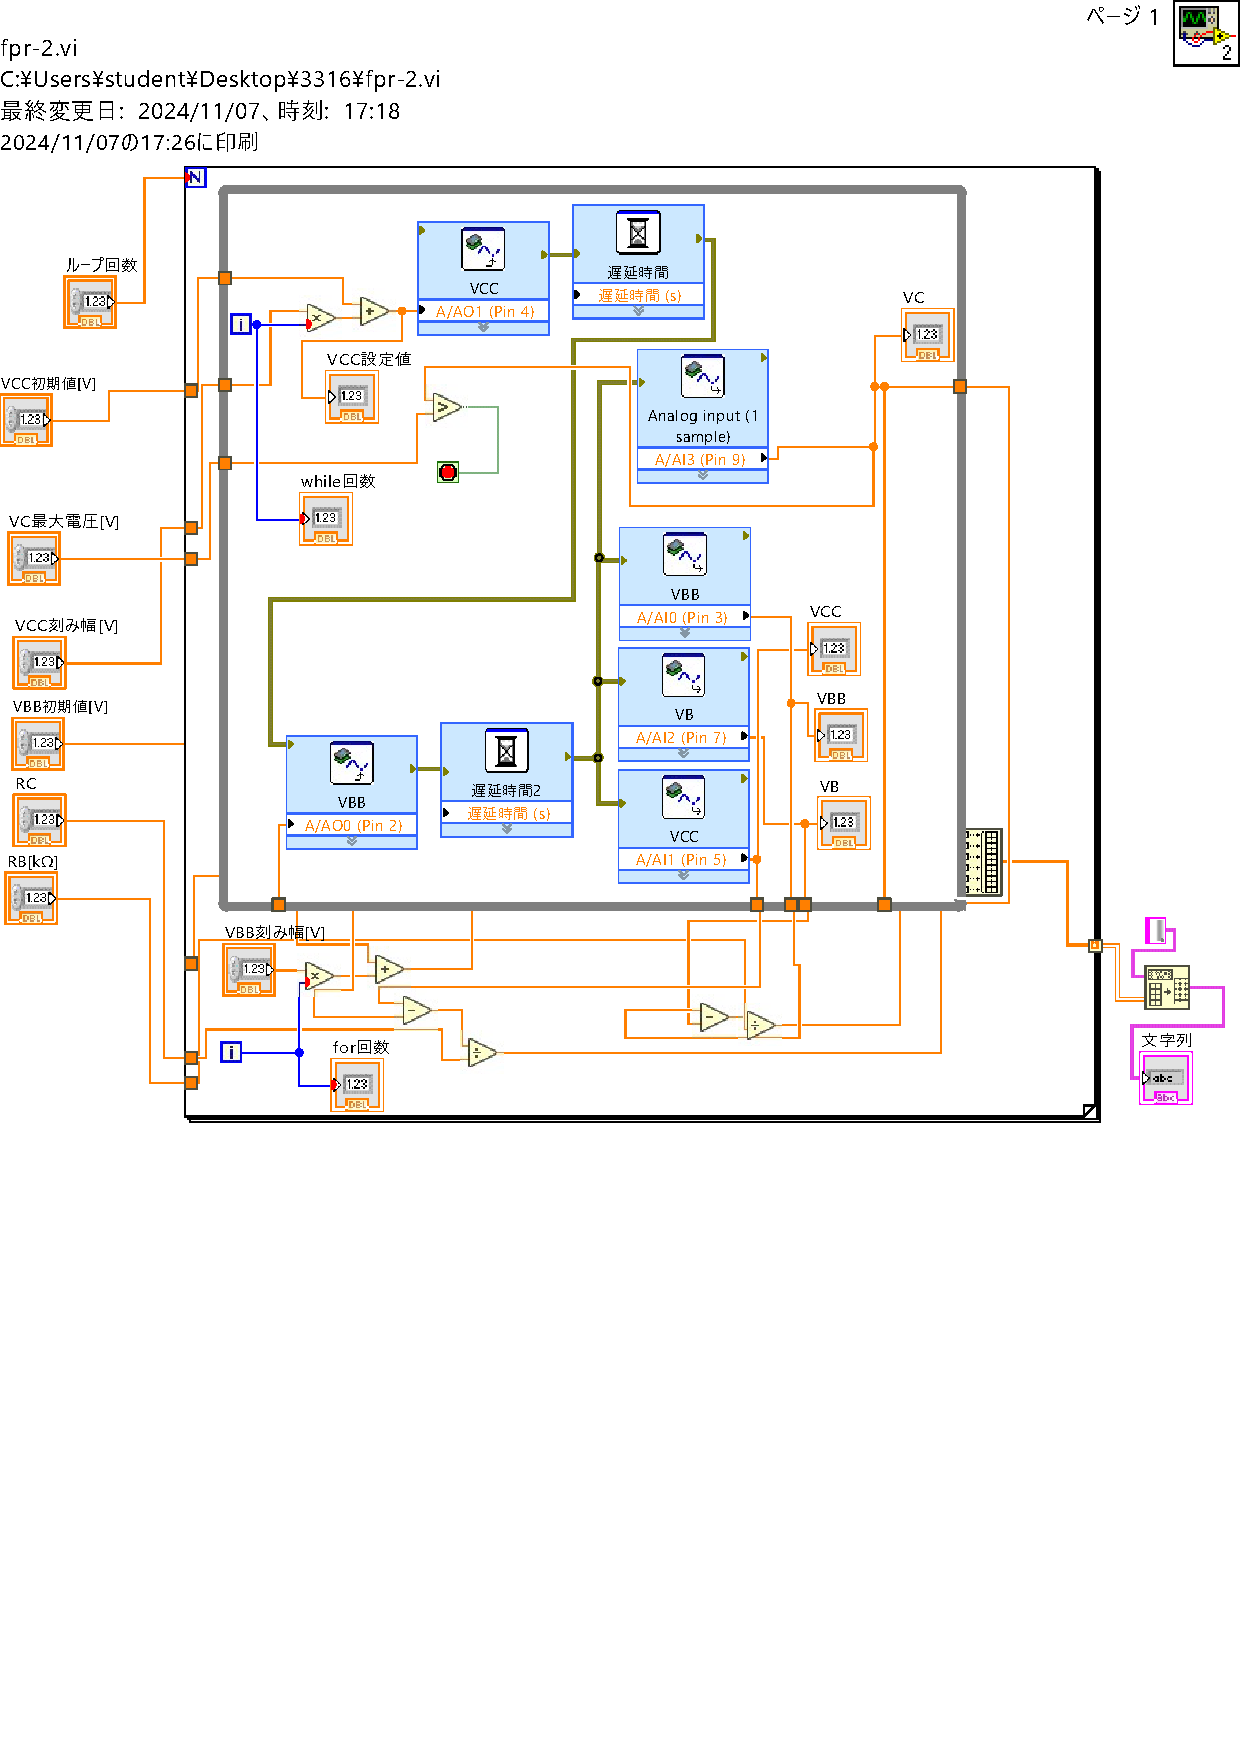
\includegraphics[scale=0.3]{fig/for-2.pdf}
				\caption{電流伝達特性測定プログラム}
				\label{fig:電流伝達特性測定プログラム}
			\end{figure}
			\item プログラムを実行し、$I_B$と$I_C$がほぼ比例しているものの、$V_C$が一定値になっていないことを確認した。
			\item 上述のプログラムを別名で保存し、以下の要領で$V_C$を一定に保つように修正した。
			\begin{itemize}
				\item $V_{BB}$を変化させているforループの中にwhileループを作成する。
				\item whileループ中で$V_{CC}$を 4 V から 0.002 V ずつ変化させ、$V_C$ を測定。
				\item $V_{CC}$の初期値、刻み幅は数値制御器または数値定数(DBL)で設定する。
				\item $V_C$が 4 V を超えたらwhileループを抜ける。
			\end{itemize}
			\item 実行し、測定結果をExcelで処理し、電流伝達特性図として描画した。
		\end{enumerate}
	\subsection{BJTの電圧帰還特性}
	\label{sec:BJTの電圧帰還特性}
	\begin{enumerate}
		\item 測定回路には\wsec{BJT電流伝達特性}にて用いたものと同様のものを使用した。
		\item \wfig{電圧帰還特性測定プログラム/出力特性測定プログラム}に示すプログラムを組んだ。
		\item $I_B$を 8 $\mu$A に一定に保ちながら$V_{CC}$を 0 V から 5 V まで、 0.2 V 刻みで変化させ測定を行った。
		\item 測定結果をExcelで処理し、電圧帰還特性として描画した。
	\end{enumerate}
	\subsection{BJTの出力特性}
	\begin{enumerate}
		\item \wfig{電圧帰還特性測定プログラム/出力特性測定プログラム}に示すコードを用いて、$I_B$が 4 $\mu$A,12 $\mu$A に設定し測定を行った。
		\item $\wsec{BJTの電圧帰還特性}$で測定したデータと合わせた3組のデータをExcelを用いて出力図として描画した。
	\end{enumerate}
\section{結果}
	\subsection{自動測定のプログラム}
		\subsubsection{入力特性測定プログラム}
		入力特性の自動測定プログラムとその出力結果を\wfig{入力特性測定プログラム},\wtab{入力特性測定結果}に示す。
		\begin{figure}[H]
			\centering
			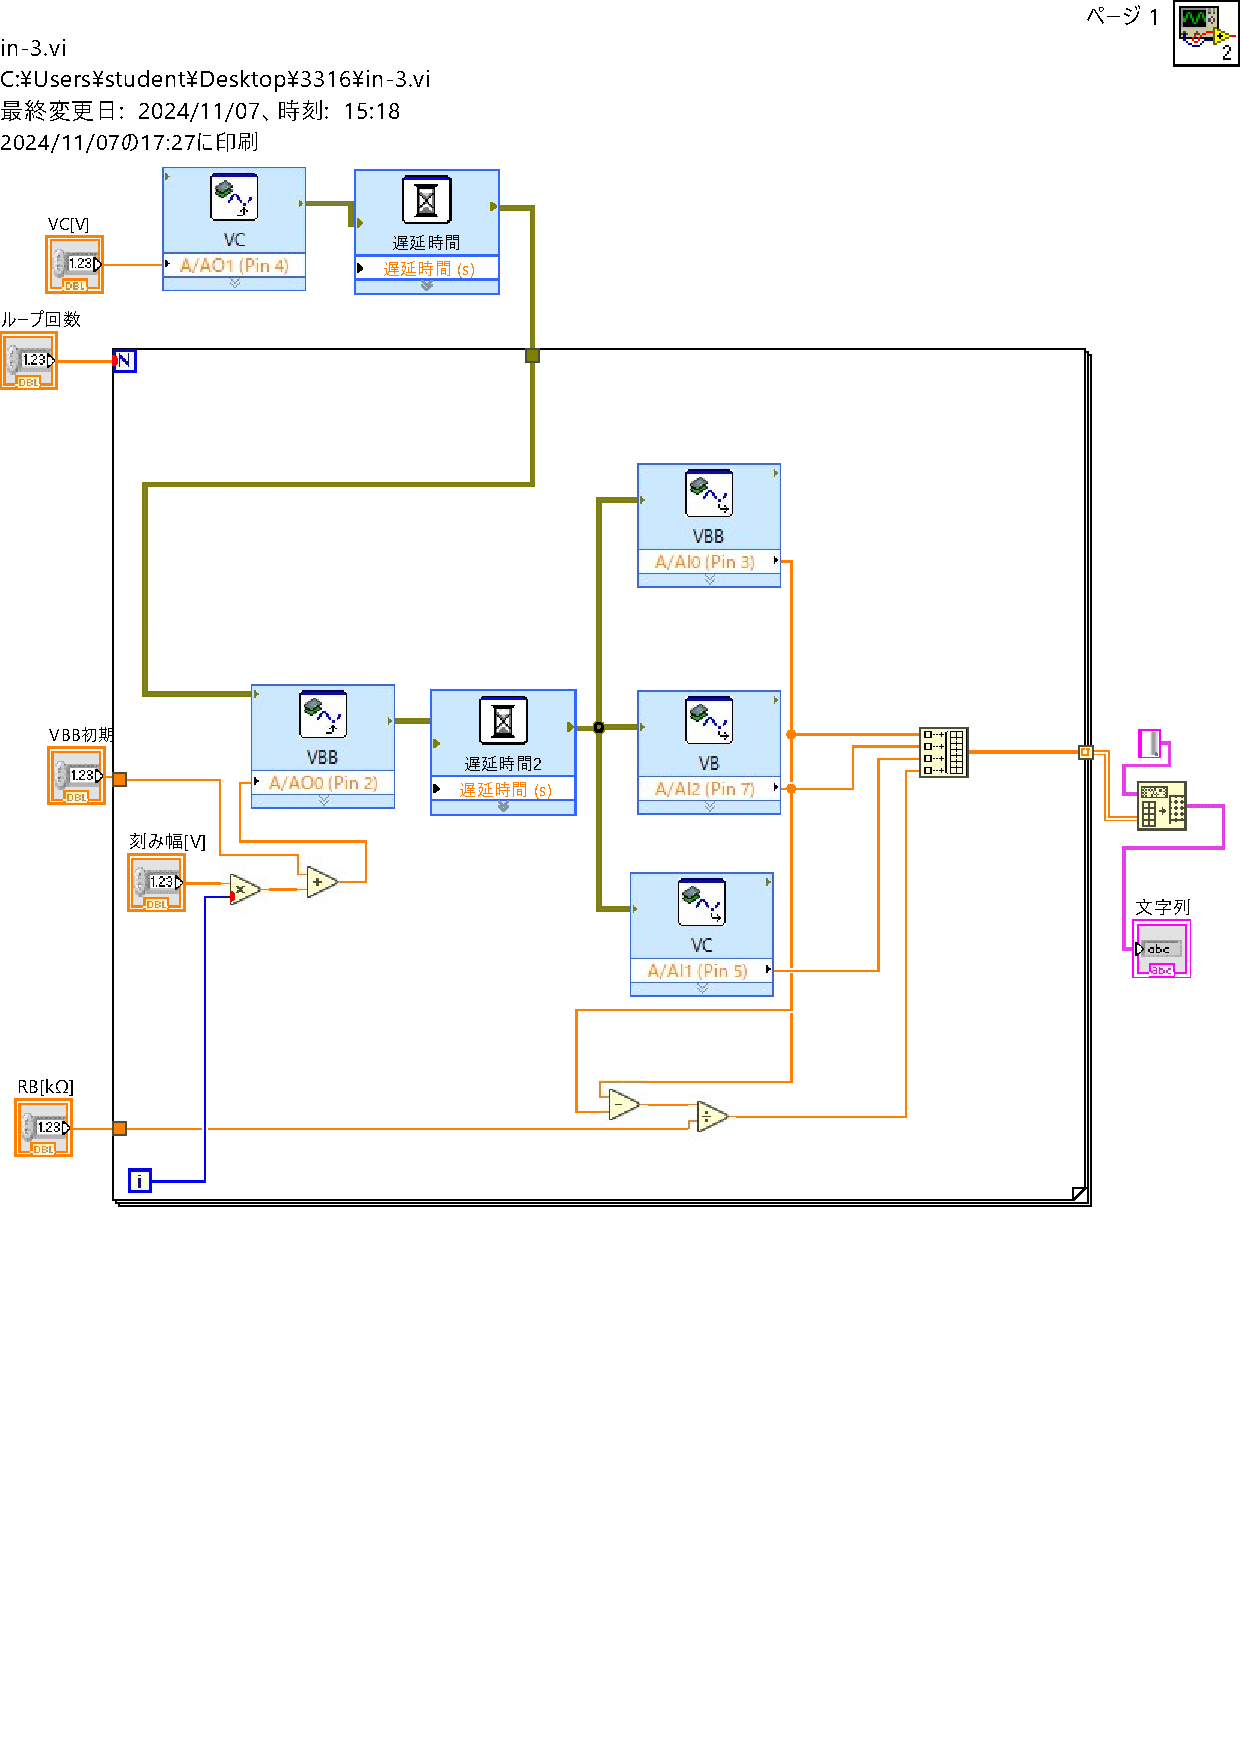
\includegraphics[scale=0.3]{fig/in-3.pdf}
			\caption{入力特性測定プログラム}
			\label{fig:入力特性測定プログラム}
		\end{figure}
		\begin{table}[H]
			\centering
			\caption{入力特性測定結果}
			\begin{tabular}{cccc}
			\hline
			$V_{BB}$ [V] & $V_B$ [V]& $V_C$ [V]& $I_B$ [mA]\\ \hline\hline
			0.008545 & 0.308838 & 4.000244 & -0.003003 \\
			0.196533 & 0.461426 & 3.997802 & -0.002649 \\
			0.395508 & 0.528564 & 4.001464 & -0.001331 \\
			0.599365 & 0.549316 & 4.000244 & 0.0005 \\
			0.79834 & 0.559082 & 3.999023 & 0.002393 \\
			0.998535 & 0.565185 & 3.999023 & 0.004333 \\
			1.19751 & 0.570068 & 4.001464 & 0.006274 \\
			1.398926 & 0.574951 & 3.997802 & 0.00824 \\
			1.5979 & 0.579834 & 4.000244 & 0.010181 \\
			1.796875 & 0.583496 & 4.001464 & 0.012134 \\
			1.99707 & 0.585937 & 4.001464 & 0.014111 \\
			2.197265 & 0.5896 & 4.001464 & 0.016077 \\
			2.397461 & 0.592041 & 4.001464 & 0.018054 \\
			2.598877 & 0.594482 & 4.000244 & 0.020044 \\
			2.797851 & 0.596924 & 4.001464 & 0.022009 \\
			2.998047 & 0.599365 & 4.000244 & 0.023987 \\
			3.198242 & 0.601807 & 4.001464 & 0.025964 \\
			3.399658 & 0.603027 & 3.999023 & 0.027966 \\
			\hline
			\end{tabular}
			\label{tab:入力特性測定結果}
		\end{table}
		\wtab{入力特性測定結果}より$V_{BB}$が上昇するにつれ$V_B$,$I_B$も上昇していることがわかる。
		\subsubsection{電流伝達特性測定プログラム}
		電流伝達特性の自動測定プログラムとその出力結果を\wfig{電流伝達特性測定プログラム},\wtab{電流伝達特性測定結果}に示す。
		\begin{figure}[H]
			\centering
			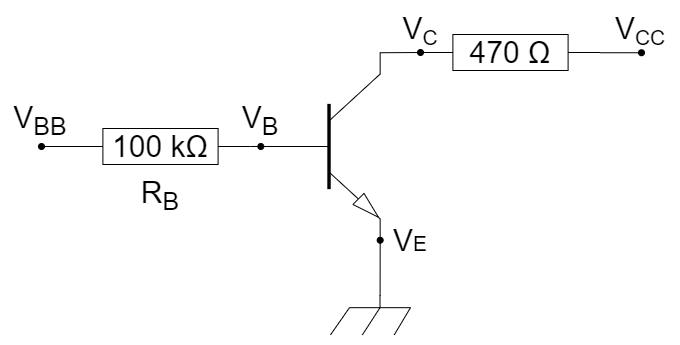
\includegraphics[scale=0.3]{fig/BJT電流伝達特性測定回路.drawio.png}
			\caption{電流伝達特性測定回路}
			\label{fig:電流伝達特性測定回路}
		\end{figure}
		\begin{table}[H]
			\centering
			\caption{電流伝達特性測定結果}
			\begin{tabular}{cccccc}
			\hline
			$V_B$ [V] & $V_{BB}$ [V]& $V_{CC} [V]$ & $I_B$ [mA]& $V_C$ [V]& $I_C$ [A]\\ \hline\hline
			0.008545 & 0.305176 & 4.001464 & -0.002966 & 3.996582 & 0.000010 \\
			0.100098 & 0.385742 & 4.001464 & -0.002856 & 3.999023 & 0.000005 \\
			0.196533 & 0.466309 & 4.002685 & -0.002698 & 4.000244 & 0.000005 \\
			0.296631 & 0.544434 & 4.000244 & -0.002478 & 3.997802 & 0.000005 \\
			0.397949 & 0.601807 & 4.001464 & -0.002039 & 3.990478 & 0.000023 \\
			0.499268 & 0.632324 & 4.002685 & -0.001331 & 3.944091 & 0.000125 \\
			0.596924 & 0.648193 & 4.000244 & -0.000513 & 3.862304 & 0.000293 \\
			0.697021 & 0.657959 & 4.001464 & 0.000391 & 3.770752 & 0.000491 \\
			0.79834 & 0.664062 & 3.999023 & 0.001343 & 3.677978 & 0.000683 \\
			0.897217 & 0.667725 & 3.999023 & 0.002295 & 3.583984 & 0.000883 \\
			0.997314 & 0.670166 & 3.999023 & 0.003271 & 3.485107 & 0.001093 \\
			1.097412 & 0.673828 & 3.997802 & 0.004236 & 3.391113 & 0.001291 \\
			1.19751 & 0.676269 & 3.999023 & 0.005212 & 3.292236 & 0.001504 \\
			1.297607 & 0.678711 & 3.997802 & 0.006189 & 3.188476 & 0.001722 \\
			1.397705 & 0.681152 & 3.996582 & 0.007166 & 3.087158 & 0.001935 \\
			1.497803 & 0.683594 & 4.019775 & 0.008142 & 3.000488 & 0.002169 \\
			1.5979 & 0.684814 & 4.149169 & 0.009131 & 3.001709 & 0.002441 \\
			1.697998 & 0.687256 & 4.293212 & 0.010107 & 3.000488 & 0.002750 \\
			1.798096 & 0.688476 & 4.466552 & 0.011096 & 3.001709 & 0.003117 \\
			\hline
			\end{tabular}
			\label{tab:電流伝達特性測定結果}
		\end{table}
		\wtab{電流伝達特性測定結果}より$V_B$が上昇するにつれ、$V_BB$、$I_B$、$I_C$が上昇していることがわかる。
		\subsubsection{電圧帰還特性測定プログラム}
		電圧帰還特性の自動測定プログラムとその出力結果を\wfig{電圧帰還特性測定プログラム/出力特性測定プログラム},\wtab{電圧帰還特性測定結果}に示す。
		\begin{figure}[H]
			\centering
			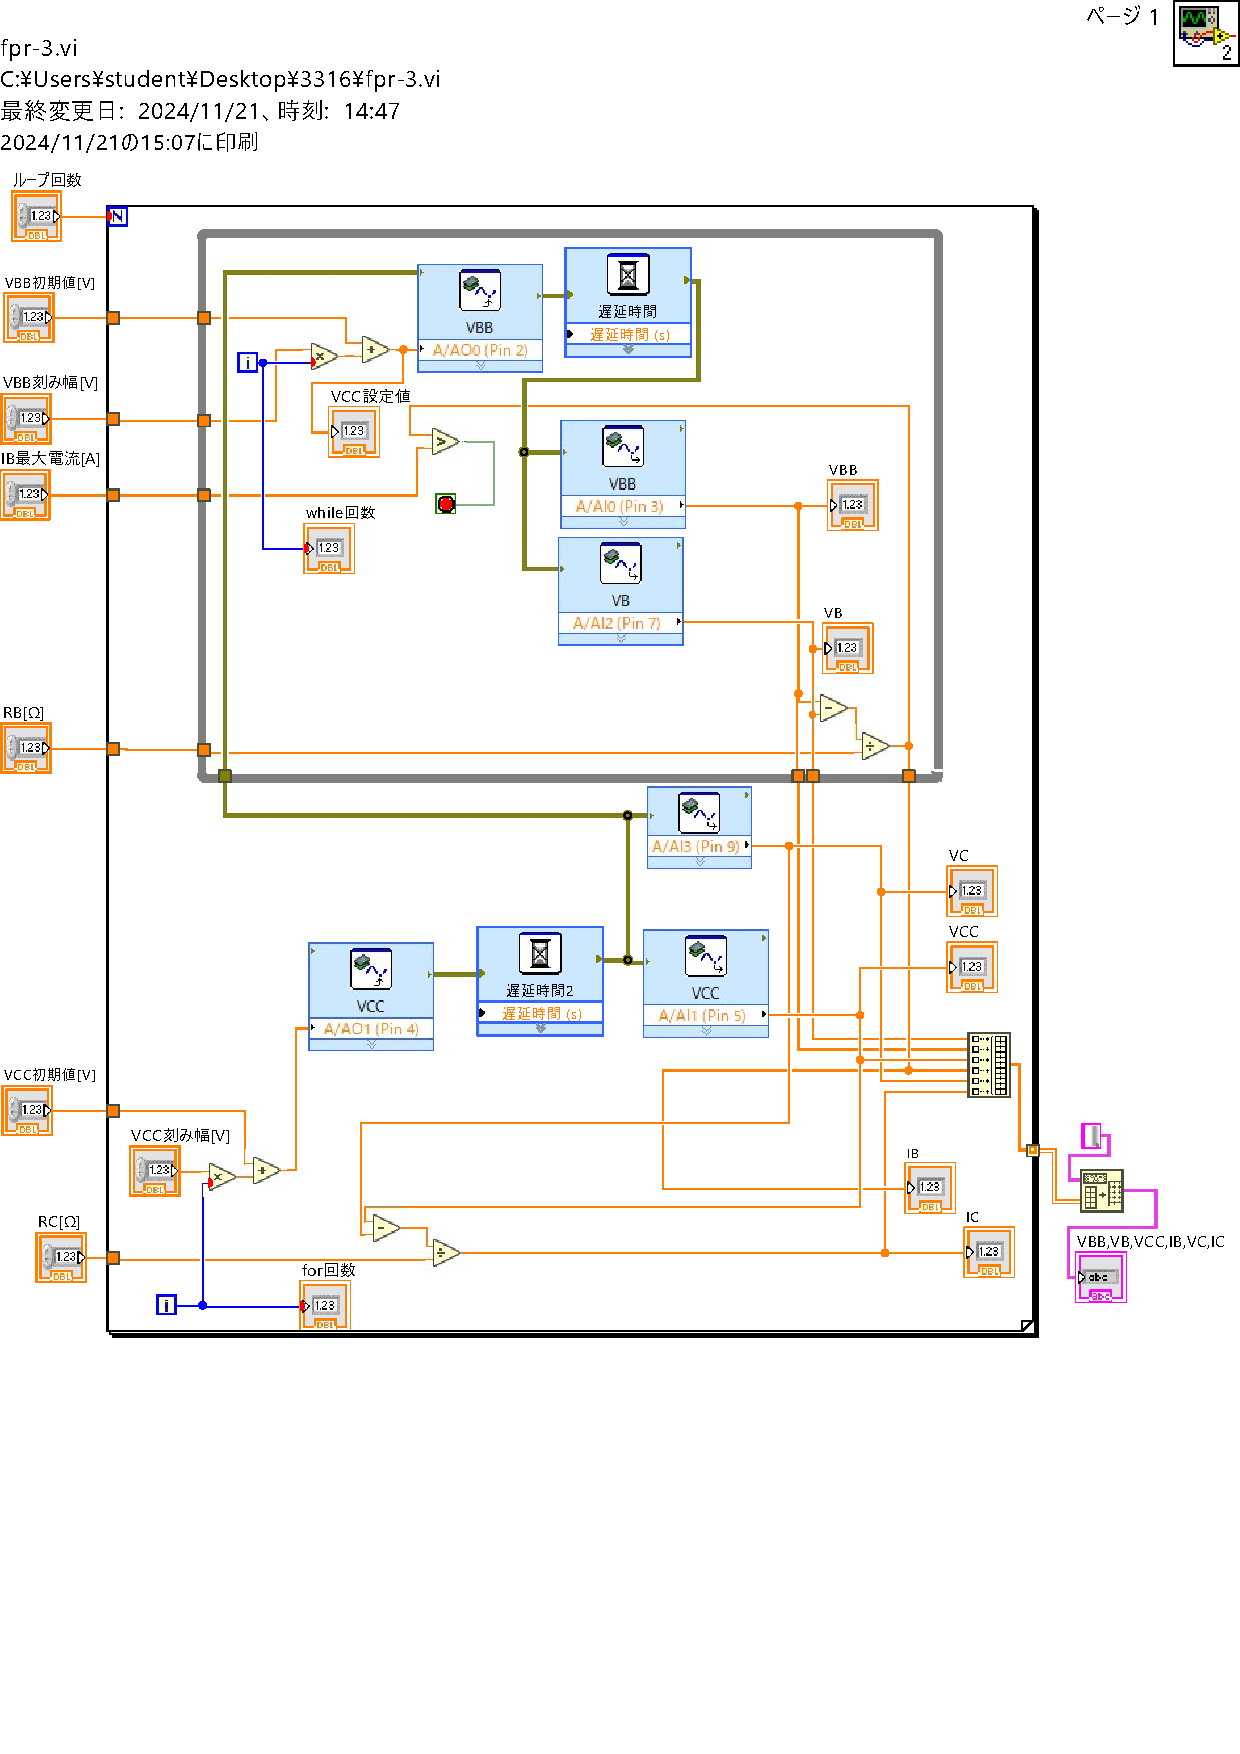
\includegraphics[scale=0.3]{fig/for-3.pdf}
			\caption{電圧帰還特性測定プログラム/出力特性測定プログラム}
			\label{fig:電圧帰還特性測定プログラム/出力特性測定プログラム}
		\end{figure}
		\begin{table}[H]
			\centering
			\caption{電圧帰還特性測定結果}
			\begin{tabular}{cccccc}
			\hline
			$V_B$ [V]& $V_{BB}$ [V]& $V_{CC}$ [V]& $I_B$ [mA]& $V_C$ [V]& $I_C$ [A]\\\hline\hline
			1.357422 & 0.554199 & 0.006104 & 0.0000080 & 0.006104 & 0.0000000 \\
			1.422119 & 0.621338 & 0.198975 & 0.0000080 & 0.073242 & 0.0002680 \\
			1.448974 & 0.64331 & 0.397949 & 0.0000081 & 0.101318 & 0.0006310 \\
			1.459961 & 0.655518 & 0.596924 & 0.0000080 & 0.128174 & 0.0009970 \\
			1.468506 & 0.662842 & 0.795898 & 0.0000081 & 0.195312 & 0.0012780 \\
			1.469726 & 0.666504 & 0.996094 & 0.0000080 & 0.349121 & 0.0013770 \\
			1.473389 & 0.667725 & 1.195068 & 0.0000081 & 0.426025 & 0.0016360 \\
			1.472168 & 0.668945 & 1.395264 & 0.0000080 & 0.612793 & 0.0016650 \\
			1.473389 & 0.670166 & 1.59668 & 0.0000080 & 0.915527 & 0.0014490 \\
			1.473389 & 0.672607 & 1.796875 & 0.0000080 & 1.107178 & 0.0014670 \\
			1.479492 & 0.672607 & 1.995849 & 0.0000081 & 1.296387 & 0.0014880 \\
			1.478271 & 0.673828 & 2.196045 & 0.0000080 & 1.489258 & 0.0015040 \\
			1.478271 & 0.675049 & 2.39624 & 0.0000080 & 1.683349 & 0.0015170 \\
			1.477051 & 0.676269 & 2.597656 & 0.0000080 & 1.875 & 0.0015380 \\
			1.478271 & 0.67749 & 2.796631 & 0.0000080 & 2.065429 & 0.0015560 \\
			1.483154 & 0.67749 & 2.996826 & 0.0000081 & 2.25708 & 0.0015740 \\
			1.479492 & 0.678711 & 3.1958 & 0.0000080 & 2.445068 & 0.0015970 \\
			1.484375 & 0.679932 & 3.395996 & 0.0000080 & 2.626953 & 0.0016360 \\
			1.485596 & 0.681152 & 3.597412 & 0.0000080 & 2.8125 & 0.0016700 \\
			1.484375 & 0.682373 & 3.796386 & 0.0000080 & 2.999267 & 0.0016960 \\
			1.484375 & 0.683594 & 3.996582 & 0.0000080 & 3.044433 & 0.0020260 \\
			1.486816 & 0.683594 & 4.197998 & 0.0000080 & 3.221435 & 0.0020780 \\
			1.489258 & 0.683594 & 4.395752 & 0.0000081 & 3.391113 & 0.0021380 \\
			1.488037 & 0.684814 & 4.595947 & 0.0000080 & 3.728027 & 0.0018470 \\
			1.490478 & 0.684814 & 4.796142 & 0.0000081 & 3.902587 & 0.0019010 \\
			1.489258 & 0.686035 & 4.995117 & 0.0000080 & 3.997802 & 0.0021220 \\
			\hline
			\end{tabular}
			\label{tab:電圧帰還特性測定結果}
		\end{table}
		\wtab{電圧帰還特性測定結果}より$V_B$が上昇するにつれ、$V_{BB}$、$V_{CC}$、$V_C$、$I_C$が上昇していることがわかる。
		\subsubsection{出力特性測定プログラム}
		出力特性の自動測定プログラムとその結果を\wfig{電圧帰還特性測定プログラム/出力特性測定プログラム},\wtab{出力特性測定結果4},\wtab{出力特性測定結果8}\wtab{出力特性測定結果12}に示す。
		\begin{table}[H]
			\centering
			\caption{出力特性測定結果($I_B$=4\ $\mu$A)}
			\begin{tabular}{cccccc}
			\hline
			$V_B$ [V]& $V_{BB}$ [V]& $V_{CC}$ [V]& $I_B$ [mA]& $V_C$ [V]& $I_C$ [A]\\\hline\hline
			0.997314 & 0.535889 & 0.007324 & 0.0000046 & 0.006104 & 2.60E-06 \\
			1.019287 & 0.615234 & 0.198975 & 0.0000040 & 0.091553 & 0.000229 \\
			1.04126 & 0.638428 & 0.397949 & 0.0000040 & 0.150146 & 0.000527 \\
			1.048584 & 0.64331 & 0.599365 & 0.0000041 & 0.244141 & 0.000756 \\
			1.052246 & 0.646973 & 0.797119 & 0.0000041 & 0.428467 & 0.000784 \\
			1.048584 & 0.648193 & 0.998535 & 0.0000040 & 0.661621 & 0.000717 \\
			1.053467 & 0.651855 & 1.19751 & 0.0000040 & 0.848389 & 0.000743 \\
			1.057129 & 0.654297 & 1.398926 & 0.0000040 & 1.040039 & 0.000764 \\
			1.063232 & 0.656738 & 1.5979 & 0.0000041 & 1.229248 & 0.000784 \\
			1.064453 & 0.65918 & 1.798096 & 0.0000041 & 1.367187 & 0.000917 \\
			1.062012 & 0.6604 & 1.998291 & 0.0000040 & 1.613769 & 0.000818 \\
			1.063232 & 0.661621 & 2.198486 & 0.0000040 & 1.80542 & 0.000836 \\
			1.066894 & 0.664062 & 2.398681 & 0.0000040 & 1.999512 & 0.000849 \\
			1.069336 & 0.665283 & 2.597656 & 0.0000040 & 2.193603 & 0.00086 \\
			1.069336 & 0.667725 & 2.799072 & 0.0000040 & 2.387695 & 0.000875 \\
			1.071777 & 0.668945 & 2.998047 & 0.0000040 & 2.520752 & 0.001016 \\
			1.070557 & 0.670166 & 3.197021 & 0.0000040 & 2.773437 & 0.000901 \\
			1.072998 & 0.672607 & 3.397216 & 0.0000040 & 2.961425 & 0.000927 \\
			1.074219 & 0.673828 & 3.599853 & 0.0000040 & 3.148193 & 0.000961 \\
			1.079101 & 0.675049 & 3.798828 & 0.0000040 & 3.339843 & 0.000977 \\
			1.079101 & 0.676269 & 3.997802 & 0.0000040 & 3.533935 & 0.000987 \\
			1.077881 & 0.67749 & 4.199218 & 0.0000040 & 3.725586 & 0.001008 \\
			1.077881 & 0.67749 & 4.398193 & 0.0000040 & 3.914795 & 0.001029 \\
			1.082764 & 0.678711 & 4.597167 & 0.0000040 & 4.104003 & 0.001049 \\
			1.082764 & 0.679932 & 4.796142 & 0.0000040 & 4.293212 & 0.00107 \\
			1.081543 & 0.681152 & 4.997558 & 0.0000040 & 4.475097 & 0.001112 \\
			\hline
			\end{tabular}
			\label{tab:出力特性測定結果4}
		\end{table}
		\begin{table}[H]
			\centering
			\caption{出力特性測定結果($I_B$=8\ $\mu$A)}
			\begin{tabular}{cccccc}
			\hline
			$V_B$ [V]& $V_{BB}$ [V]& $V_{CC}$ [V]& $I_B$ [mA]& $V_C$ [V]& $I_C$ [A]\\\hline\hline
			1.357422 & 0.554199 & 0.006104 & 0.0000080 & 0.006104 & 0.0000000 \\
			1.422119 & 0.621338 & 0.198975 & 0.0000080 & 0.073242 & 0.0002680 \\
			1.448974 & 0.64331 & 0.397949 & 0.0000081 & 0.101318 & 0.0006310 \\
			1.459961 & 0.655518 & 0.596924 & 0.0000080 & 0.128174 & 0.0009970 \\
			1.468506 & 0.662842 & 0.795898 & 0.0000081 & 0.195312 & 0.0012780 \\
			1.469726 & 0.666504 & 0.996094 & 0.0000080 & 0.349121 & 0.0013770 \\
			1.473389 & 0.667725 & 1.195068 & 0.0000081 & 0.426025 & 0.0016360 \\
			1.472168 & 0.668945 & 1.395264 & 0.0000080 & 0.612793 & 0.0016650 \\
			1.473389 & 0.670166 & 1.59668 & 0.0000080 & 0.915527 & 0.0014490 \\
			1.473389 & 0.672607 & 1.796875 & 0.0000080 & 1.107178 & 0.0014670 \\
			1.479492 & 0.672607 & 1.995849 & 0.0000081 & 1.296387 & 0.0014880 \\
			1.478271 & 0.673828 & 2.196045 & 0.0000080 & 1.489258 & 0.0015040 \\
			1.478271 & 0.675049 & 2.39624 & 0.0000080 & 1.683349 & 0.0015170 \\
			1.477051 & 0.676269 & 2.597656 & 0.0000080 & 1.875 & 0.0015380 \\
			1.478271 & 0.67749 & 2.796631 & 0.0000080 & 2.065429 & 0.0015560 \\
			1.483154 & 0.67749 & 2.996826 & 0.0000081 & 2.25708 & 0.0015740 \\
			1.479492 & 0.678711 & 3.1958 & 0.0000080 & 2.445068 & 0.0015970 \\
			1.484375 & 0.679932 & 3.395996 & 0.0000080 & 2.626953 & 0.0016360 \\
			1.485596 & 0.681152 & 3.597412 & 0.0000080 & 2.8125 & 0.0016700 \\
			1.484375 & 0.682373 & 3.796386 & 0.0000080 & 2.999267 & 0.0016960 \\
			1.484375 & 0.683594 & 3.996582 & 0.0000080 & 3.044433 & 0.0020260 \\
			1.486816 & 0.683594 & 4.197998 & 0.0000080 & 3.221435 & 0.0020780 \\
			1.489258 & 0.683594 & 4.395752 & 0.0000081 & 3.391113 & 0.0021380 \\
			1.488037 & 0.684814 & 4.595947 & 0.0000080 & 3.728027 & 0.0018470 \\
			1.490478 & 0.684814 & 4.796142 & 0.0000081 & 3.902587 & 0.0019010 \\
			1.489258 & 0.686035 & 4.995117 & 0.0000080 & 3.997802 & 0.0021220 \\
			\hline
			\end{tabular}
			\label{tab:出力特性測定結果8}
		\end{table}
		\begin{table}[H]
			\centering
			\caption{出力特性測定結果($I_B$=12\ $\mu$A)}
			\begin{tabular}{cccccc}
			\hline
			$V_B$ [V]& $V_{BB}$ [V]& $V_{CC}$ [V]& $I_B$ [mA]& $V_C$ [V]& $I_C$ [A]\\\hline\hline
			1.773681 & 0.571289 & 0.007324 & 0.0000120 & 0.006104 & 2.60E-06 \\
			1.831055 & 0.629883 & 0.197754 & 0.0000120 & 0.073242 & 0.000265 \\
			1.850586 & 0.649414 & 0.395508 & 0.0000120 & 0.085449 & 0.00066 \\
			1.864013 & 0.661621 & 0.598144 & 0.0000120 & 0.13916 & 0.000977 \\
			1.871338 & 0.670166 & 0.795898 & 0.0000120 & 0.123291 & 0.001431 \\
			1.876221 & 0.675049 & 0.996094 & 0.0000120 & 0.357666 & 0.001358 \\
			1.882324 & 0.679932 & 1.195068 & 0.0000120 & 0.177002 & 0.002166 \\
			1.883545 & 0.682373 & 1.395264 & 0.0000120 & 0.253906 & 0.002428 \\
			1.885986 & 0.684814 & 1.595459 & 0.0000120 & 0.927734 & 0.001421 \\
			1.889648 & 0.684814 & 1.795654 & 0.0000120 & 1.119385 & 0.001439 \\
			1.887207 & 0.686035 & 1.993408 & 0.0000120 & 0.805664 & 0.002527 \\
			1.888428 & 0.686035 & 2.194824 & 0.0000120 & 1.500244 & 0.001478 \\
			1.887207 & 0.686035 & 2.395019 & 0.0000120 & 1.690674 & 0.001499 \\
			1.888428 & 0.687256 & 2.595215 & 0.0000120 & 1.879883 & 0.001522 \\
			1.889648 & 0.687256 & 2.794189 & 0.0000120 & 2.072754 & 0.001535 \\
			1.889648 & 0.688476 & 2.995605 & 0.0000120 & 2.263183 & 0.001558 \\
			1.89209 & 0.689697 & 3.193359 & 0.0000120 & 1.911621 & 0.002727 \\
			1.89331 & 0.689697 & 3.394775 & 0.0000120 & 2.078857 & 0.0028 \\
			1.894531 & 0.690918 & 3.59497 & 0.0000120 & 2.247314 & 0.002867 \\
			1.89209 & 0.690918 & 3.795166 & 0.0000120 & 3.010254 & 0.00167 \\
			1.89209 & 0.690918 & 3.995361 & 0.0000120 & 3.193359 & 0.001706 \\
			1.89331 & 0.692139 & 4.195556 & 0.0000120 & 3.378906 & 0.001738 \\
			1.89331 & 0.690918 & 4.39331 & 0.0000120 & 3.558349 & 0.001777 \\
			1.89331 & 0.692139 & 4.592285 & 0.0000120 & 3.739013 & 0.001815 \\
			1.894531 & 0.690918 & 4.79248 & 0.0000120 & 3.908691 & 0.00188 \\
			1.89331 & 0.690918 & 4.991455 & 0.0000120 & 4.077148 & 0.001945 \\
			\hline
			\end{tabular}
			\label{tab:出力特性測定結果12}
		\end{table}
		\wtab{出力特性測定結果4}、\wtab{出力特性測定結果8},\wtab{出力特性測定結果12}より$V_B$が上昇するにつれ、$V_{BB}$、$V_{CC}$、$V_C$、$I_C$が上昇していることがわかる。
	\subsection{特性図}
		\subsubsection{入力特性}
		入力特性の特性図を\wfig{入力特性図}に示す。
		\begin{figure}[H]
			\centering
			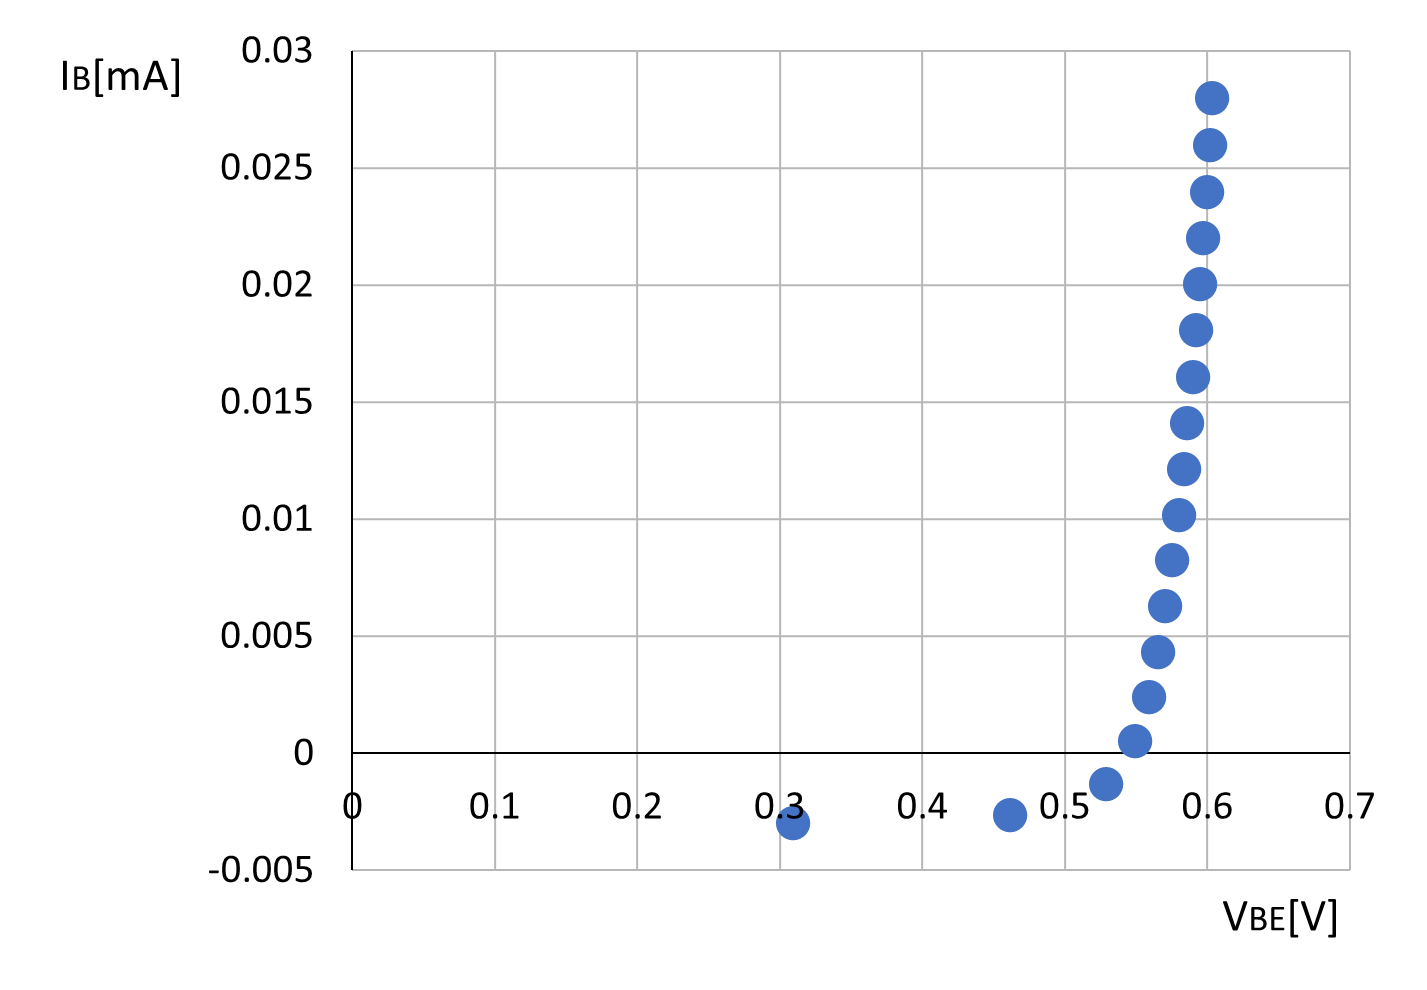
\includegraphics[scale=0.8]{fig/入力特性図.png}
			\caption{入力特性図}
			\label{fig:入力特性図}
		\end{figure}
		\wfig{入力特性図}よりこのトランジスタは$v_{BE} = 0.6$V 付近で電流を流すようになることが分かる。
		\subsubsection{電流伝達特性}
		電流伝達特性の特性図を\wfig{電流伝達特性図}に示す。
		\begin{figure}[H]
			\centering
			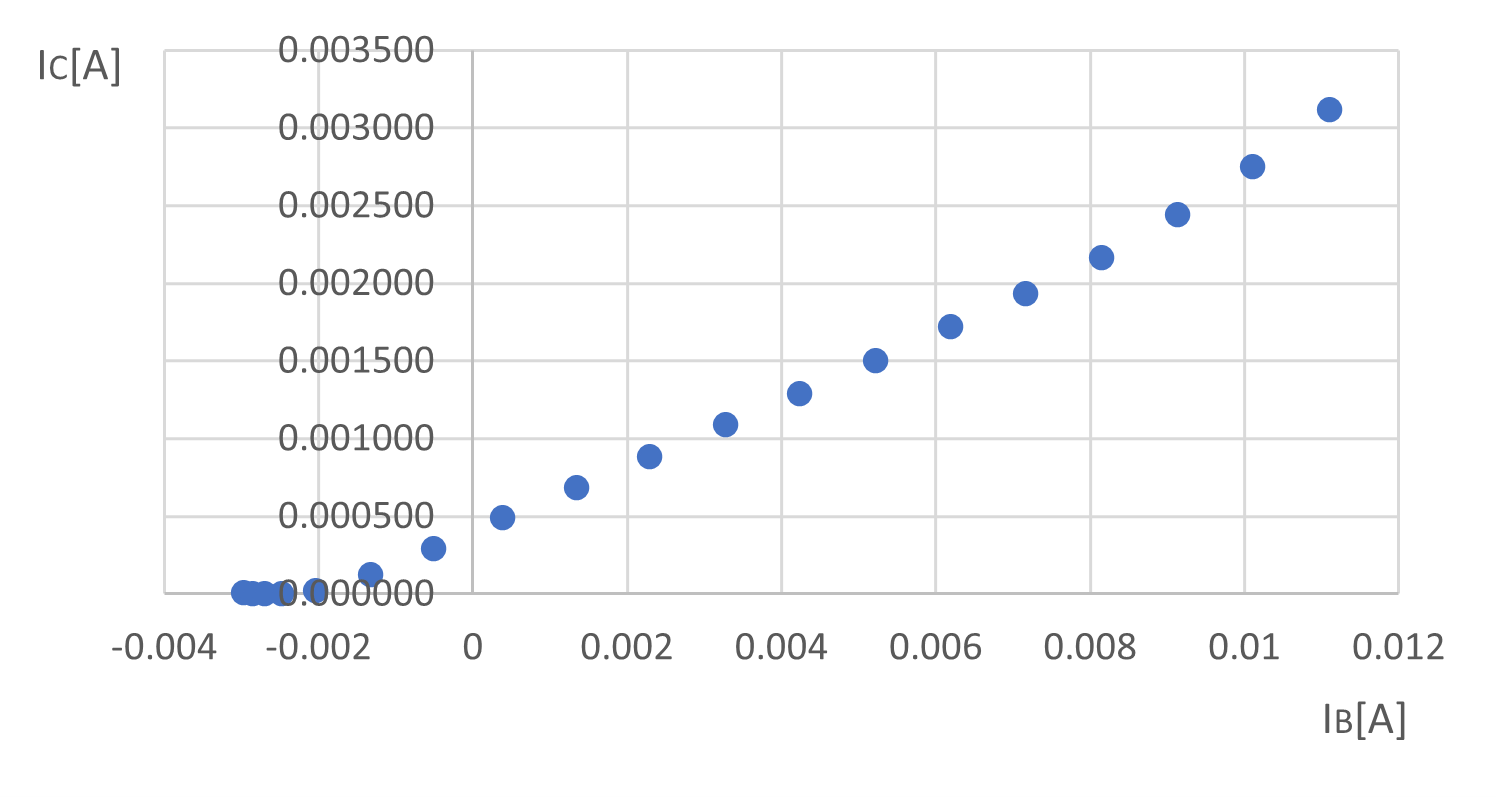
\includegraphics[scale=0.8]{fig/電流伝達特性図.png}
			\caption{電流伝達特性図}
			\label{fig:電流伝達特性図}
		\end{figure}
		\wfig{電流伝達特性図}より$i_B = -0.002$A 付近から電流$I_C$が上昇し始めることがわかる。
		\subsubsection{電圧帰還特性}
		電圧帰還特性の特性図を\wfig{電圧帰還特性図}に示す。
		\begin{figure}[H]
			\centering
			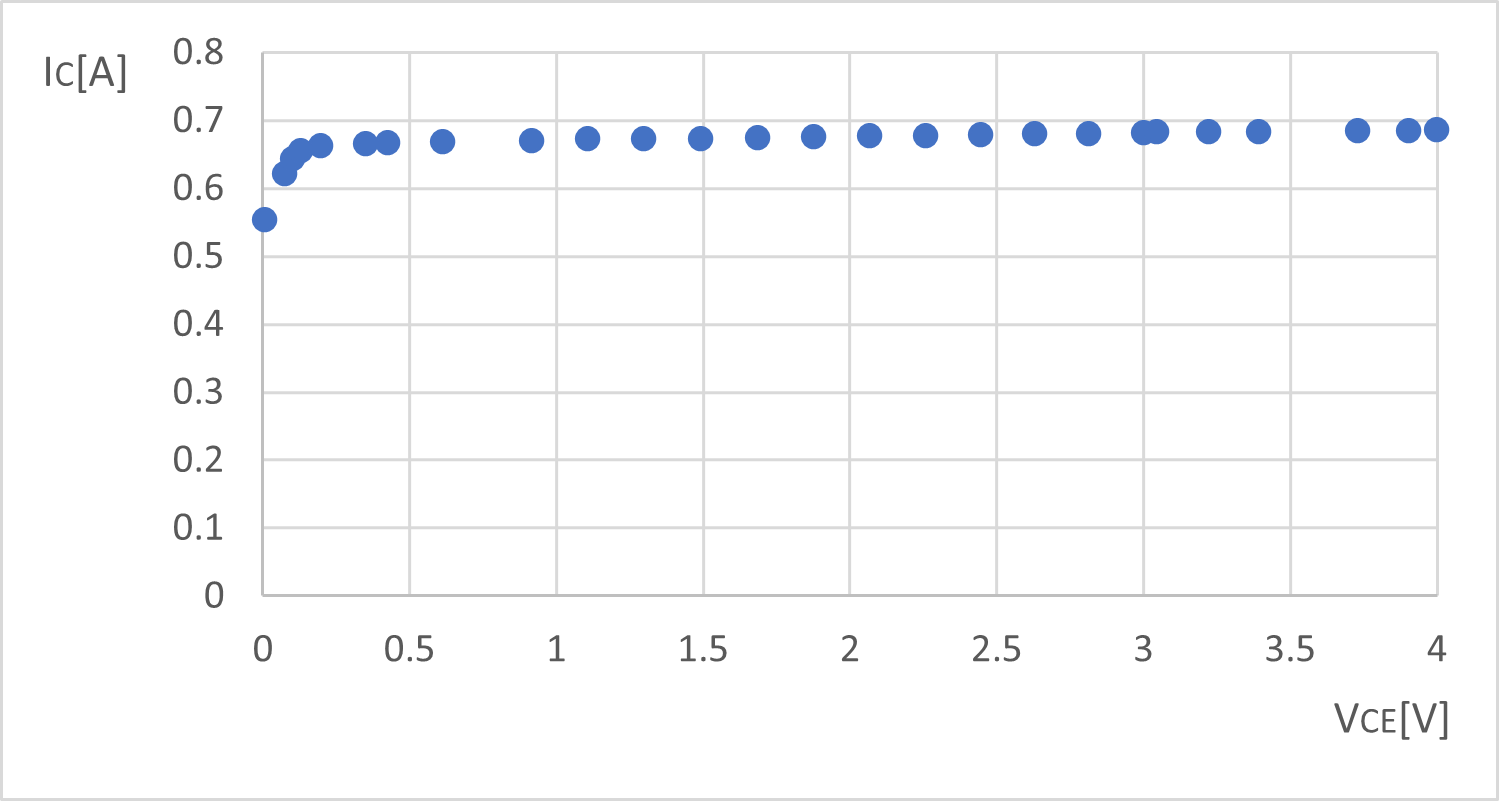
\includegraphics[scale=0.8]{fig/電圧帰還特性図.png}
			\caption{電圧帰還特性図}
			\label{fig:電圧帰還特性図}
		\end{figure}
		\wfig{電圧帰還特性図}より$i_C = 0.7$ A 付近で漸近していることが分かる。
		\subsubsection{出力特性}
		出力特性の特性図を\wfig{出力特性図}に示す。
		\begin{figure}[H]
			\centering
			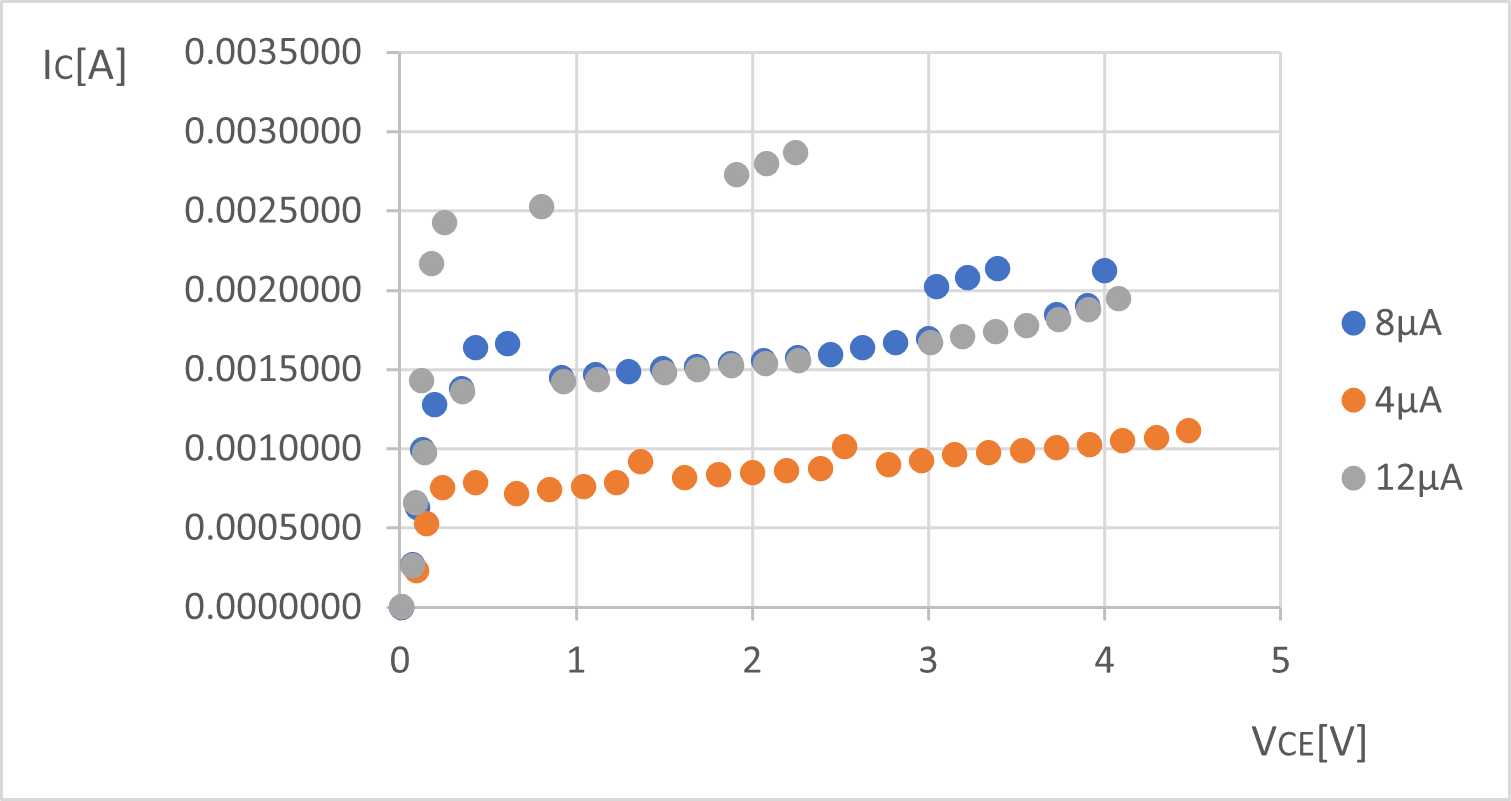
\includegraphics[scale=0.8]{fig/出力特性図.png}
			\caption{出力特性図}
			\label{fig:出力特性図}
		\end{figure}
		\wfig{出力特性図}より$i_B = 12 \mu$A及び$i_B = 8 \mu$Aの値の一部において$i_C$異常な値が検知されていることが分かる。
\section{考察}
	\subsection{Hパラメータの導出}
	\label{sec:Hパラメータの導出}
		\subsubsection{最小二乗法}
		Hパラメータは各グラフの傾きより求められる。
		しかし計測値には誤差が含まれ綺麗な綺麗なグラフにならず、傾きが求められない。
		そこで今回は最小二乗法によりy=ax+bに近似してHパラメータを求める。
		今回用いる式を\weq{最小二乗法}に示す。
		\begin{eqnarray}
			\left\{ \,
			\begin{aligned}
				\frac{1}{n}\sum_{i = 6}^{n}(y_i-y)^2=0\\
				y=ax_i+b\\
			\end{aligned}
			\right.\nonumber\\
			\frac{1}{n}\sum_{i = 1}^{n}(y_i-(ax_i+b))^2 &=& 0\nonumber\\
			a &=& \frac{n\sum_{i = 6}^{n}x_iy_i-\sum_{i = 1}^{n}y_i\sum_{i = 1}^{n}x_i}{n\sum_{i = 1}^{n}x^2-(\sum_{i = 1}^{n}x)^2}
			\label{eq:最小二乗法}
		\end{eqnarray}
		\subsubsection{入力インピーダンス($h_{ie}$)}
		入力インピーダンス($h_{ie}$)は\weq{最小二乗法}より以下の式で求められる。
		\begin{eqnarray}
			h_{ie} &=& \frac{\Delta V_{BE}}{\Delta I_B}\nonumber\\
			&=& \frac{1}{a}\nonumber\\
			&=& \frac{n\sum_{i = 1}^{n}V_B^2-(\sum_{i = 1}^{n}V_B)^2}{n\sum_{i = 1}^{n}V_BI_B-\sum_{i = 1}^{n}I_B\sum_{i = 1}^{n}V_B}\ \Omega
			\label{eq:hieの導出}
		\end{eqnarray}
		よって、\wtab{入力特性測定結果}より$30.9$ [k$\Omega$]と求まる。
		\subsubsection{電流増幅率($h_{fe}$)}
		電流増幅率$h_{fe}$は以下の式で求められる。
		\begin{eqnarray}
			h_{fe} &=& \frac{\Delta I_C}{\Delta I_B} \nonumber\\
			&=& \frac{n\sum_{i = 1}^{n}I_CI_B-\sum_{i = 1}^{n}I_C\sum_{i = 1}^{n}I_B}{n\sum_{i = 1}^{n}I_B^2-(\sum_{i = 1}^{n}I_B)^2}
			\label{eq:hfeの導出}
		\end{eqnarray}
		よって、\wtab{電流伝達特性測定結果}より$2.14*10^2$と求まる。
		\subsubsection{電圧帰還率($h_{re}$)}
		電圧帰還率($h_{re}$)は以下の式で求められる。
		\begin{eqnarray}
			h_{re} &=& \frac{\Delta V_{BE}}{\Delta V_{CE}} \nonumber\\
			&=& \frac{n\sum_{i = 1}^{n}V_BV_C-\sum_{i = 1}^{n}V_B\sum_{i = 1}^{n}V_C}{n\sum_{i = 1}^{n}V_C^2-(\sum_{i = 1}^{n}V_C)^2}
		\end{eqnarray}
		よって、\wtab{電圧帰還特性測定結果}より31.0と求まる。
		\subsubsection{出力アドミタンス($h_{oe}$)}
		出力アドミタンス($h_{oe}$)は以下の式で求められる。
		\begin{eqnarray}
			h_{oe} &=& \frac{\Delta I_C}{\Delta V_{CE}} \nonumber\\
			&=& \frac{n\sum_{i = 1}^{n}I_CV_C-\sum_{i = 1}^{n}I_C\sum_{i = 1}^{n}V_C}{n\sum_{i = 1}^{n}V_C^2-(\sum_{i = 1}^{n}V_C)^2}\ S
			\end{eqnarray}
		よって、\wtab{出力特性測定結果4}より$1.97*10^{-4}$ Sと求まる。
	\subsection{Hパラメータの測定結果について}
		\subsubsection{入力インピーダンス($h_{ie}$)}
		\wsec{Hパラメータの導出}より今回の測定では$h_{ie}$は $1.48$ k$\Omega$と求められている。
		今回実験に用いたトランジスタ2N3904の$h_{ie}$は 0 $\approx$ 2.2 k$\Omega$のため、この値は少し小さいが妥当であると考えられる。
		\subsubsection{電流増幅率($h_{fe}$)}
		\wsec{Hパラメータの導出}より今回の測定では$h_{fe}$は $233$ と求められている。
		今回実験に用いたトランジスタの$h_{fe}$は最大で 300 程度になるため、この値は妥当であると考えられる。
		\subsubsection{電圧帰還率($h_{re}$)}
		\wsec{Hパラメータの導出}より今回の測定では$h_{re}$は $0.0000515$ と求められている。
		今回実験に用いたトランジスタの$h_{re}$は $5*10^{-5}$ 程度になるため、この値は妥当であると考えられる。
		\subsubsection{出力アドミタンス($h_{oe}$)}
		\wsec{Hパラメータの導出}より今回の測定では$h_{oe}$は $88$ $\mu$Sと求められている。
		今回実験に用いたトランジスタの$h_{oe}$は 9 $\mu$Sであるため、この値は大きすぎると考えられる。
	\subsection{測定値が飛び飛びの値しかない理由}
	今回の実験ではmyRIOを用いて測定を行った。
	myRIOはその特性上アナログ計器と異なり分解能の上限が存在する。
	そのため、連続した値ではなく、測定値が飛び飛びの値しかない。
	\subsection{HパラメータからYパラメータへの変換}
	HパラメータからYパラメータは\weq{HパラメータからYパラメータへの変換}に示す式で行える。
	\begin{eqnarray}
		\begin{pmatrix}i_1\\i_2\end{pmatrix} &=& \begin{pmatrix}\frac{1}{H_{11}}&-\frac{H_{12}}{H_{11}}\\\frac{H_{21}}{H_{11}}&\frac{H_{11}H_{22}-H_{12}H_{21}}{H_{11}}\end{pmatrix}\begin{pmatrix}i_1\\v_2\end{pmatrix}
		\label{eq:HパラメータからYパラメータへの変換}
	\end{eqnarray}
	\weq{HパラメータからYパラメータへの変換}に今回の測定値を代入すると
	\begin{eqnarray}
		\begin{pmatrix}Y_{11}&Y_{12}\\Y_{21}&Y_{22}\end{pmatrix} &=& \begin{pmatrix}6.75*10^{-4}&-3.47*10^{-8}\\0.1574&3.764*10^{-5}\end{pmatrix}
		\label{eq:HパラメータによるYパラメータ}
	\end{eqnarray}
	\subsection{独自の考察}
	\wfig{出力特性図}において異常な値が検知された原因として$i_C$が既定の値まで上昇しきっていないというのが考えられる。
\section{結論}
\begin{itemize}
	\item トランジスタの入力/出力/電流伝達/電圧機関の諸特性図の概形が描けるようになった
	\item トランジスタの特性図が、hパラメータを求める方法を理解した
	\item 電圧と電流の関係式から、等価回路を求める方法を理解した
	\item LabVIEWを用いて、2端子対回路の電圧と電流を自動測定する方法を理解した
\end{itemize}
\begin{thebibliography}{9}
\bibitem{a}
\end{thebibliography}

\end{document}

